\documentclass[12pt]{article}
\usepackage{amsfonts}
\usepackage{hyperref}
\usepackage{setspace}
\usepackage{graphicx}
\usepackage{gensymb}
\usepackage{moresize}
\begin{document}

\newpage
{\Large \section{Introduction}}

Automation in industries is the need of the hour. Everything is done electrically and not manually, right from a really unnoticed process like moving the conveyors to something as power intensive as running pumps. Industrial automation is primarily necessary for high end production and also product quality controls. Mainly, in industries, such automations are carried out by intelligent systems called Programmable Logic Controllers with the help of a host computer. A PLC, is in an actual sense, an electrical version of a microcontroller unit. It's more generic and also controls high power tools which generally work at really high voltages, unlike the microcontroller that merely works at considerably small voltage values. Basically, it intelligently controls whatever is programmed onto it by the host computer. This controller, being so versatile, is highly expensive, due to it's high rising demand and also it's operability credits.  \singlespace
\vspace{12pt}
A PLC generally has a set of input and output ports to with the external peripherals are connected, which are to be electrically controlled by the PLC. Looking into the flow of working of the PLC, the processor tries to make decisions in accordance to the program, generally written by the user using some logic used to program these units. Some of these logics include \texttt{Function Block Diagram, Ladder Diagram, Structured Text, Sequential Function Chart} and \texttt{Instruction List}.\singlespace
\vspace{12pt}
The objective is to create an Open Source PLC, which has the capabilities of the industrial PLC, but the catch here is, it's much cheaper and simpler to work with. It incorporates a development board, that works on AVR's \texttt{ATmega16A} IC, giving upto 40 pins, most of which can be used and programmed as the Input-Output pins as it's done on a PLC. Moreover, the logic used here is \texttt{Ladder Logic} which is one of the easiest and also, robust in terms of its efficiency. Main point here is, this device is a standalone device, which can work without the host system being there, just being powered by a source. \texttt{HEX} files to be generated according to the controller are generated by a software called \texttt{LDMicro}, freely available for \texttt{Windows} and \texttt{Linux} users alike. The programming on the board is done via a \texttt{RS-232} cable by serial communication. All the processor wants now is a code to be dumped on it to start automating your small needs.\singlespace
\vspace{12pt} 
This prototype will be helpful for students to get the feel of working with the PLCs, to control small automated systems. It'll also be easy as there's no coding involved and it's using a GUI that is user friendly and also efficient. Along with the development board, which can be used as microcontroller also, there are various hardware modules to start off with and later the students can cone up with their own hardware setups and test their modules, with the board. It's really versatile as it can suit your microcontroller needs and also work as a PLC. All you need is the HEX code for your desired usage with hardware.\vspace{12pt}


The manual covers the basics of using the associated software and also explains the interfacing with the hardware. Certain simple experiments are given so as to get accustomed to the software usage. Later, some modules that can be made using the various sensors discussed in the preceding sections are covered. Then the imagination of the student and the need can drive the making of various other modules  according to the students need.

\newpage
{\Large \section{Setting up the LD Micro executable}}
Many softwares support PLC simulation in various logics.

\vspace{12pt} 

The software that has been used in the subsequent sections is \texttt{LDMicro} that incorporates \texttt{Ladder Logic}, supporting many microcontrollers, along with the AVR's \texttt{ATmega16A}. This software helps produce the HEX files according to the microcontroller and the pin selected which can be directly dumped onto the core. \vspace{24pt}

 To download the software on your \texttt{Windows} system, go to  \url{http://cq.cx/ladder.pl}. The download is a direct executable, there's no need to install it.


\begin{figure}[h!]
\centering
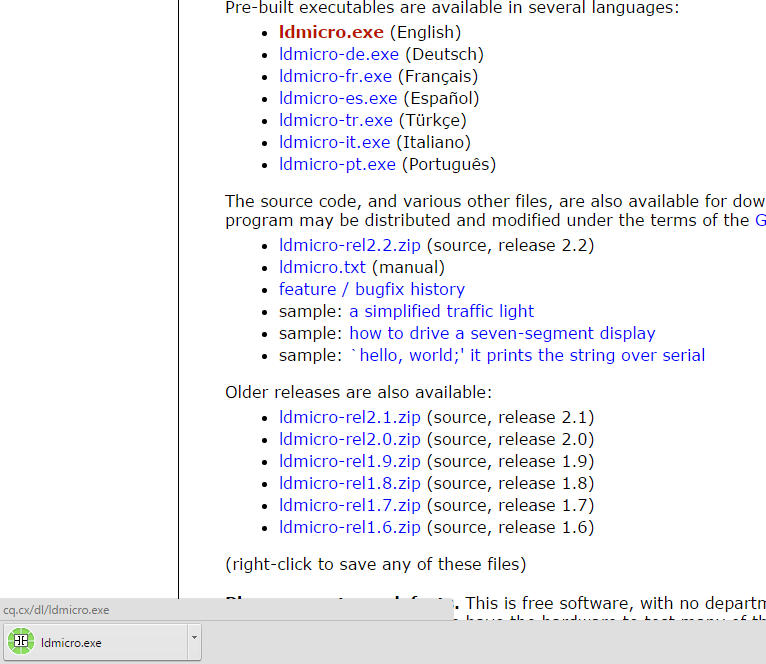
\includegraphics[scale=0.5]{screen.png}
\caption{Downloading LD Micro}
\end{figure}

\newpage


\newpage
{\Large \section{Getting started with LDMicro}}
{\large \subsection{Understanding the instructions}}
A PLC is largely programmed using \texttt{Ladder Logic}, which is used in this software. It allows us to select the microcontroller that we wish to program via its HEX codes generated, \texttt{ATmega16A} in this case. The naming convention is very intuitive and is easy to get accustomed to. Some of the naming conventions followed are:
\vspace{12pt}
\begin{enumerate}
\item \texttt{Yvar} implies the component is connected to an input pin on the microcontroller, something like a push button that is user dependent. This generally works for the digital inputs, \texttt{HIGH(+5V) or LOW(GND)}.
\item \texttt{Xvar} implies the component is connected to an output pin on the microcontroller. This can be something like an LED or a Buzzer that is used to show the outputs. It's generally used to display digital outputs, \texttt{HIGH(+5V) or LOW(GND)}.
\item \texttt{Tvar} implies, a timer. It can be a turn on, turn off or a retentive timer, just like the ones used in the actual PLCs.
\item \texttt{Cvar} implies a counter. The arguments in this are simple logical operands to decide the upper bound upto which the counter shall work. There are circular counter too, which count circularly, without any bound.
\item \texttt{Avar} implies the  values read from the Analog pins of the controller. This can be used to take the intermediate readings say from components like Potentiometers, IR sensors etc.
\end{enumerate}
\vspace{12pt}
Things to remember are :\vspace{12pt}
\begin{itemize}
\item Variable names can incorporate alphabets, numbers and underscores. It doesn't support the special characters.
\item Do not start the name of the variable with a number.
\item The variable names are case sensitive, the variable names \texttt{Relay1} and \texttt{relay1} signify two different variables.
\item The instructions such as the arithmetic ones can manipulate the variables associated with the timers, counters or input, output pins.
\item The variables are 16 bit signed decimals, so the variables can also be containing values that are negative pertaining to that range.
\item As counters, timers in physical sense are internal in the microcontroller, we can only assign the pins to the \texttt{Xname, Yname and Aname} objects and not others.
\end{itemize}
Now that the basic ideas are clear, the use of certain instructions can be discussed. 

We shall understand normally open and normally closed connections. In normally open case, the contacts are open generally, which means, giving a high input closes the contact, hereby passing the signal over the rung. Whereas, a normally closed connection would imply a high signal to the connection would break the circuit hence giving low as the output.\vspace{12pt}
\begin{enumerate} 
\item {\textbf{Contacts} are something like a prototype of a switch, which implies, if the signal going into the contact is true, only then it'll be reflected as output, if false, then output is false for normally open case.  These can be used as internal relays too. }
\item{ \textbf{Coils} are basically corresponding to the output devices. They can set the output true, if the signal going into them is true for the normally open case, else it's the other way. They can be used with internal relays too. There is an option of Set only (Reset-only) which are set(reset) when the input goes from \texttt{Low to High}, and retain their states. Hence they are used with Reset-Only(Set-Only) coils to change the states as and when wanted. }
\item{ \textbf{Internal Relays} are the ones that are never assigned pin numbers. Basically, they are the ones that are used for counters or triggers, which are not given inputs or outputs, hence no pin on the controller.}
\item{ \textbf{Turn on Delay} simply means delaying turning on of any coil. This mean the sensor, if gives a high at the input, it delays the turning on of the next part of the rung by those many units of time}
\item{ \textbf{Turn off Delay} literally means turning off of any coil with some delay. This mean the sensor, if gives a false or a low at the input, it delays the turning off of the next part of the rung by those many units of time}

\item{ \textbf{Retentive timer} is used to keep track of the how much time the module under consideration has been true, it cumulates the total time, if the input has been on for atleast that much time, the output of the timer is true. It will always reamin true after this, hence it should be reset by using \textbf{Reset} instruction manually}

\item{ \textbf{Counter} is used to count upto the given value threshold.The count is changed as the input to the counter is made high. This is used as an up counter, down counter or a circular counter. The variables can be manipulated and be suited for the application}
\item{ \textbf{Mov} is used to move any value, be it character or numeric into the variable named under destination.}
\item{ \textbf{Arithmetic operands} are used to manipulate the variables values to suit the logic, they cn be used on any kind of variables like the counters variables.}

These are the basic ones that are used. A detailed help for the more instructions and general guidelines is provided on the \texttt{Manual} of the software under the \texttt{Help} menu.
\end{enumerate} 
\newpage
{\large \subsubsection{Configuration of ATmega16A}}
\begin{figure}[h!]
\centering
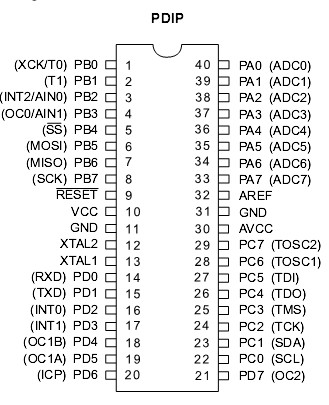
\includegraphics[scale=0.7]{atmega16.png}
\caption{ATmega16A Pin Configuration}
\end{figure}
\newpage
{\large \subsection{Creating ladders using LD Micro}}
LD Micro's simple user interface is really easy to use and is self explanatory.

To get started working with LD Micro, just double click the LD Micro executable present in your system.\vspace{12pt}
Once opened, you shall get such a GUI.\vspace{12pt}
\begin{figure}[h!]
\centering
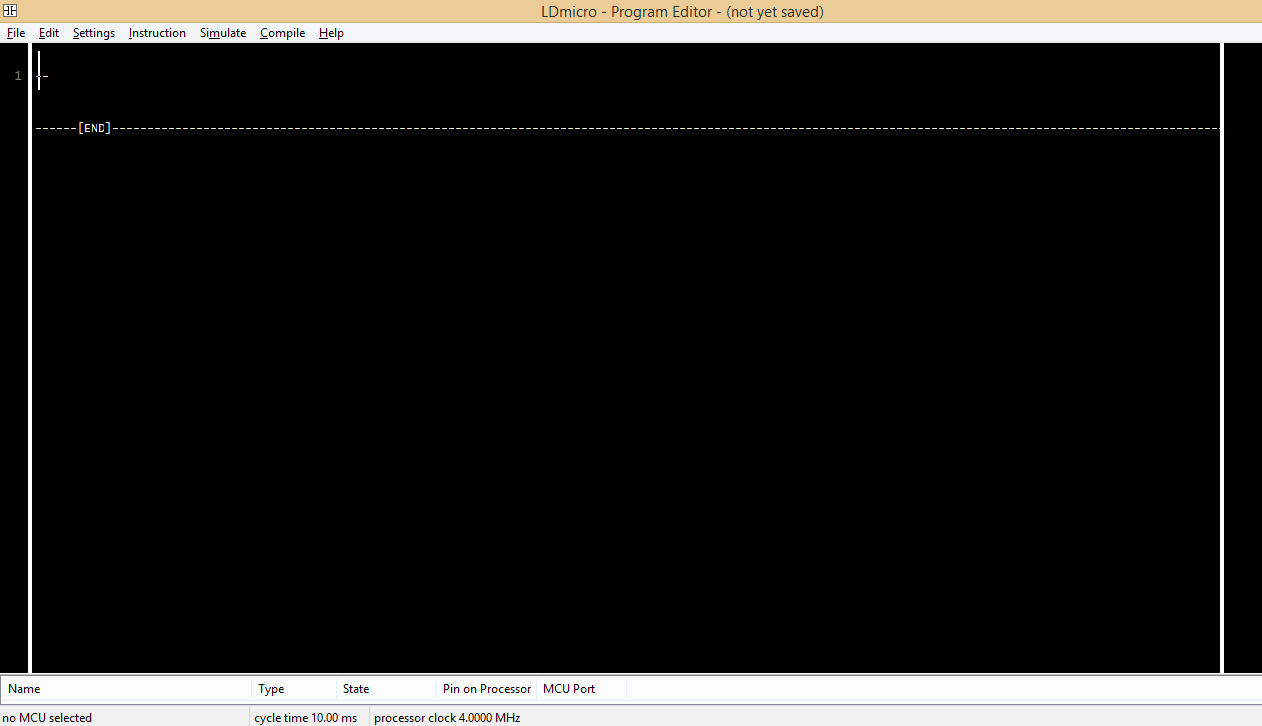
\includegraphics[scale=0.4]{ld1.png}
\caption{Startup screen of LD Micro}
\end{figure}

\vspace{12pt}Before starting to make the ladder, first make the necessary changes in the default settings, so as to generate the HEX code for your microcontroller.\vspace{12pt}
\newpage
Under \texttt{Settings} tab, select the \texttt{MCU Parameters} Option
\begin{figure}[h!]
\centering
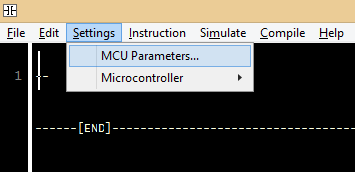
\includegraphics[scale=1]{prop.png}
\end{figure}
\begin{figure}[h!]
\centering
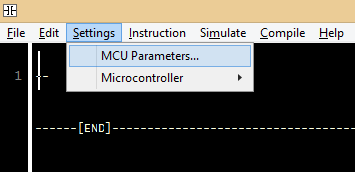
\includegraphics[scale=0.8]{Setup.png}
\caption{Changing the controller parameters}
\end{figure}
\newpage
Then after selecting, change the clock frequency to 16MHz and if using UART change the baud rate to 9600.
\begin{figure}[h!]
\centering
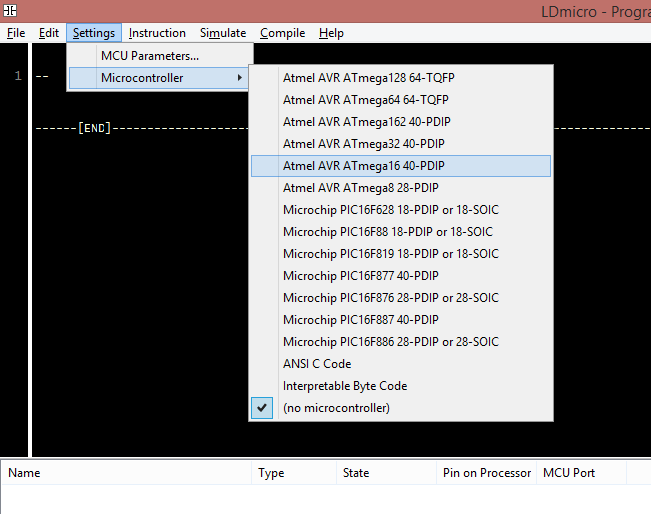
\includegraphics[scale=0.8]{cont.png}
\caption{Selecting the appropriate microcontroller}
\end{figure}
\newpage
Now that the configurations are set, the next step can be followed to design the ladder with the appropriate logic.

It's really easy to build up the Ladder, just a few clicks and you're good to go. 

Start off with having a look at the \texttt{Instruction} tab. It has a lot of instructions that are in accordance with the Ladder logic followed for the PLCs and work in the same way and are similar to the ones described above under the 'Understanding the Instructions' section. 

After selecting the appropriate instruction, just double click the instruction to edit the name of the variable and other parameters related to the particular instruction.\vspace{12pt}
\begin{figure}[h!]
\centering
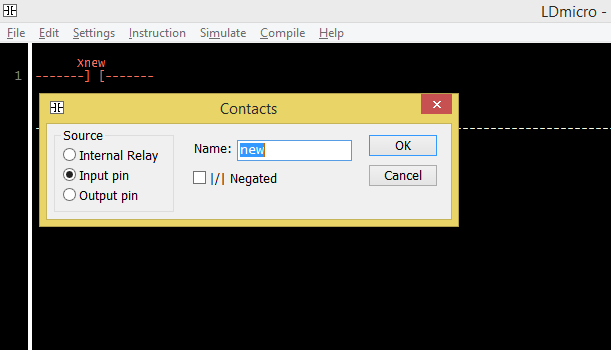
\includegraphics[scale=0.8]{change.png}
\caption{Editing the parameters of an instruction}
\end{figure}

\vspace{12pt}
\newpage
After making the appropriate ladder for the application, the digital input and outputs should be given an appropriate pin number of the controller and the connections should be done accordingly. This can be done by double clicking the appropriate pin to be configured in the consolidated table just below the ladder made.  \vspace{12pt}
\begin{figure}[h!]
\centering
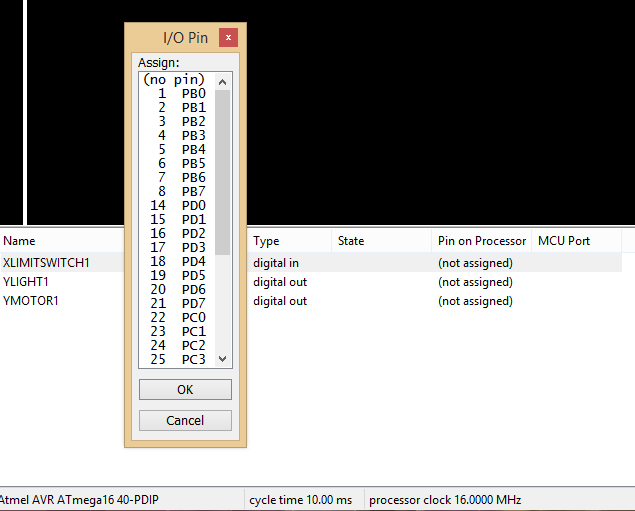
\includegraphics[scale=0.8]{PIN.png}
\caption{Assigning the appropriate pin number}
\end{figure}
\newpage
Now that the logic is set, the ladder can be simulated to verify it's working. This is done by clicking the \texttt{Simulate} tab and \texttt{Simulation Mode} option under it. This is then followed by a similar screen where \texttt{Blue} indicates \texttt{LOW} and \texttt{Pink} indicates \texttt{HIGH}. To start the simulation, under  \texttt{Simulate} tab click \texttt{Start Real-Time Simulation} option. After this, to change the state, just double click the instruction. The appropriate changes and values pertaining to different variables can be seen in the consolidated instruction table under the \texttt{State} column. To come out of simulation mode, click the same \texttt{Simulation Mode} option. \vspace{12pt}
\begin{figure}[h!]
\centering
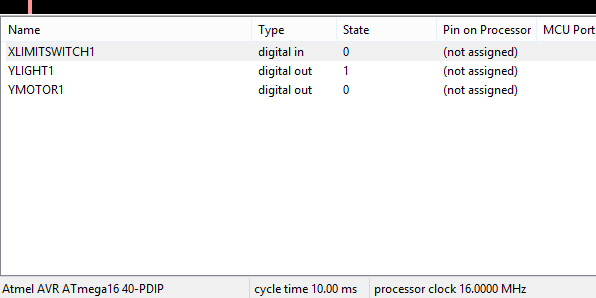
\includegraphics[scale=0.8]{states.png}
\caption{Tracking the pin states from the table}
\end{figure}

\vspace{12pt}After the ladder along with assigning the appropriate pin numbers, the HEX code can be generated. This can be done by first saving the ladder under the \texttt{File} tab with the \texttt{Save As} option. Save the file in the appropriate destination folder with a suitable name. Remember the final destination of the same for future. Now, to generate the HEX file, select the \texttt{Compile} tab and then the option \texttt{Compile As}. Then save this text file in the desired destination folder. The location shall be noted as it'd be needed to burn the code onto the controller using the command line arguments later.
\newpage{\Large \section{Programming the IC}}
{\large \subsection{Installing WINAVR}}

The IC is a standalone one without the Bootloader. One of the ways of dumping the code, is using an In System Programmer or an ISP. So, for burning the same we use the softwares:
AVRDUDE\footnote{AVRDUDE has once been started by Brian S. Dean as a private project of an in-system programmer for the Atmel AVR microcontroller series, as part of the Opensource and free software tools collection available for these controllers.} - AVR Downloader Uploader - is a program for downloading and uploading the on-chip memories of Atmel’s AVR microcontrollers. It can program the Flash and EEPROM, and where supported by the serial programming protocol, it can program fuse and lock bits. It's available as \texttt{WINAVR} for \texttt{Windows} and can be downloaded from here.
%\hyperref[WINAVR	]{''http://softlayer-sng.dl.sourceforge.net/project/winavr/WinAVR/20100110/WinAVR-20100110-install.exe''}
\linebreak
\url{http://softlayer-sng.dl.sourceforge.net/project/winavr/WinAVR/20100110/WinAVR-20100110-install.exe}\vspace{12pt}


Instead if you have \texttt{Linux} system, it's already pre-installed under the name \texttt{AVRDUDE}. Just enter the below command line on your \texttt{terminal} \vspace{12pt}

\texttt{man avrdude}

\vspace{12pt}

You would see a screen full of text, something like the one below. To exit press \texttt{q}. If you don't get a screen like that, then open \texttt{Ubuntu Software Center} and on the search bar enter \texttt{avrdude}, then install it. Enter the same command into the terminal again and you shall see the manual.

\vspace{12pt}

\begin{figure}[h!]
\centering
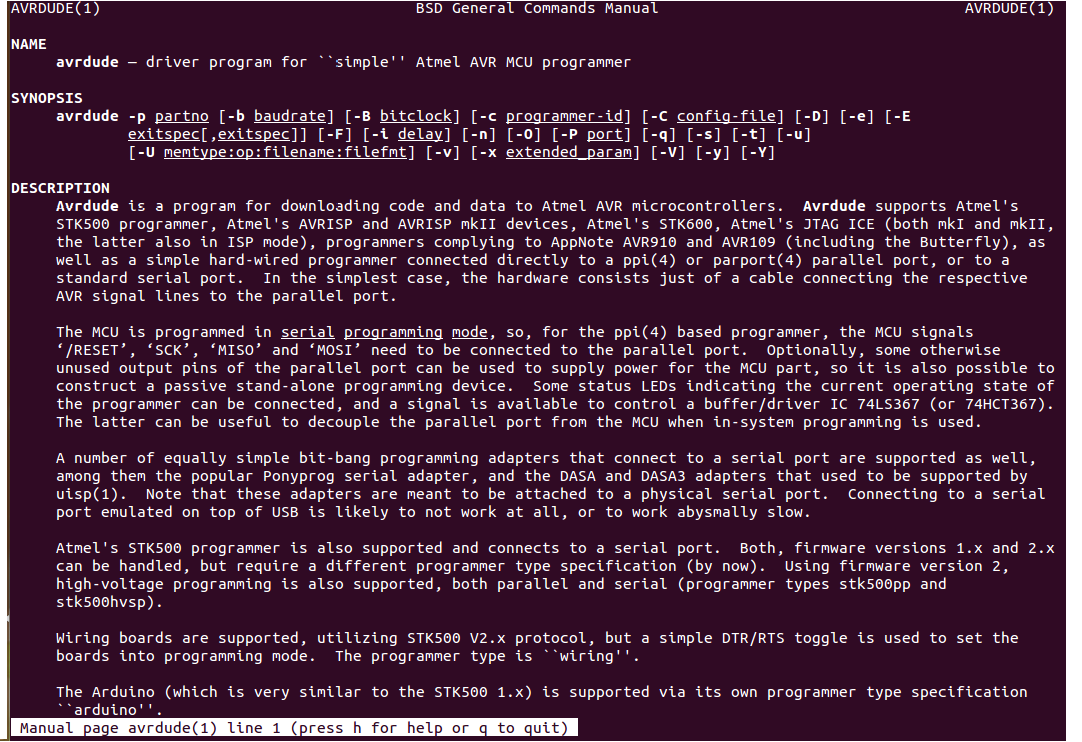
\includegraphics[scale=0.45]{manavrdude.png}
\caption{AVRDUDE manual on Linux}
\end{figure}


\clearpage

{\large \subsection{Setting up WINAVR on WINDOWS}}
Step 1: First, open up the start screen and then search : \texttt{Command Prompt}
\begin{figure}[h!]
\centering
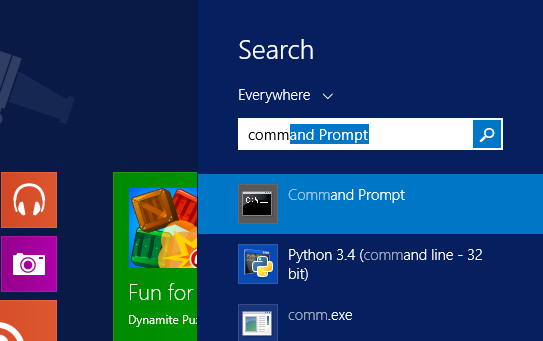
\includegraphics[scale=0.45]{Figcmd.png}
\caption{Terminal in Search screen}
\end{figure}
\linebreak
Step 2: Then, a screen like this shall pop up.

\begin{figure}[h!]
\centering
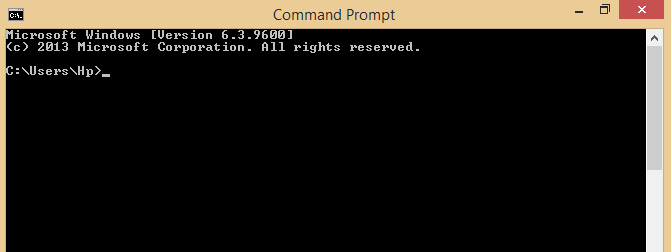
\includegraphics[scale=0.7]{Comm.png}
\caption{Terminal in use}
\end{figure}


Step 3: Enter into the command prompt for windows: \texttt{avrdude}


You should get prompts and flags mentioned like this, which implies that you have downloaded the software properly.
\begin{figure}[h]
\centering
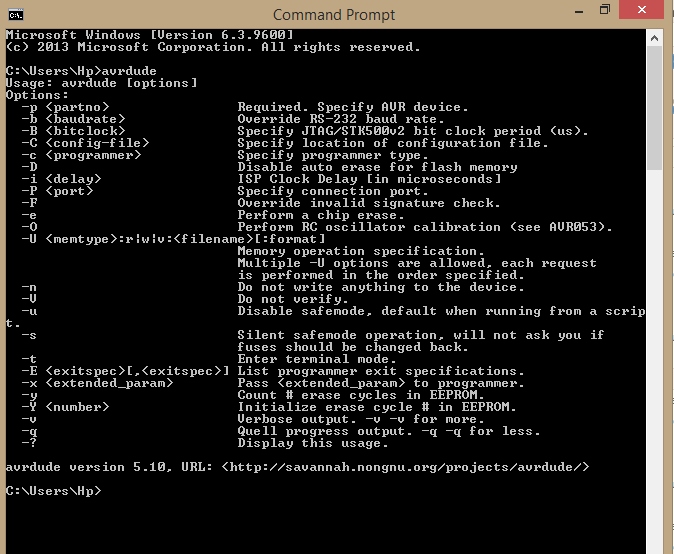
\includegraphics[scale=0.8]{avrdude1.png}
\caption{Avrdude access via WINAVR and Terminal}
\end{figure}

\pagebreak
\texttt{IMP: If you do not get this, please download the software and install it again.}\vspace{12pt}

After this, we can proceed with dumping the HEX code onto the IC.
\newpage
\subsection{Identifying the Port of the programmer}

There are several programmers available to program any controller IC. They are called as ISPs. USBASP is one of them. To identify the port at which its connected in \texttt{Linux}. \vspace{12pt}

Type into the \texttt{Terminal:}
\texttt{ls /dev}\vspace{12pt}

\begin{figure}[h!]
\centering
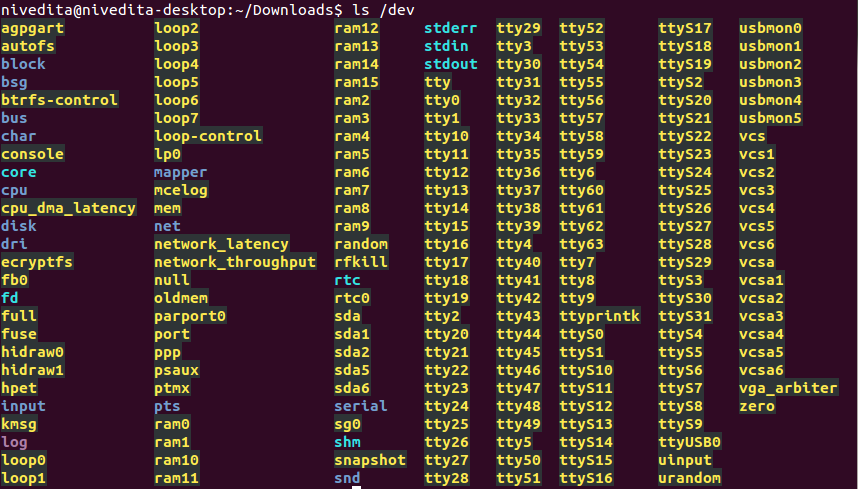
\includegraphics[scale=0.75]{device.png}
\caption{Terminal in Search screen}
\end{figure}

This gives the list of connected devices on the system. After this, connect the ISP to the system and then again enter the same command on the terminal and then find out the new entries in the list. That shall be the port at which the ISP is connected. To use it in the command line with the -P flag just mention \texttt{/dev/ttyUSBx} where the argument trailing the \texttt{/dev/} one is the port at which the device is configured. This helps in recognising the device when programming on the terminal. For example use it in the command line with the appropriate flag like this.\vspace{12pt}

\texttt{avrdude -p atmega16 -P /dev/ttyUSB0	-c ponyser -v -U flash:w:test1.hex}\vspace{12pt}

Note: It can also be used with the correct defined By-id path in the serial programming ISP(RS232) by mentioning 

\begin{verbatim}

   /dev/serial/by-id/usb-FTDI_FT232R_USB_UART_XXXXX-port0

\end{verbatim}
which is same as the\texttt{ /dev/ttyUSBx} for identifying the same programmer. So both arguments are valid in case of RS232.
\newpage\subsection{USBASP as ISP}
Step 1: We require a precompiled hex file to be burnt onto our microcontroller. In our case, we have generated it by doing simple ladder programming in LDMicro and then compiling it. Before that, ensure that the proper target controller from the drop-down menu is chosen. For input and output part, assign a certain pin no. of the controller to that of the desired application. Now, a certain name is given to the file(say, blink.hex) at the destination folder.\vspace{12pt}

Step 2: After being done with all the software part, one shall supply the power from 12V SMPS to the development board. Now check whether the controller is powered up properly with 5 Volt or not from the appropriate \texttt{Vcc} and \texttt{GND} pins of the controller.
\vspace{12pt}


Step 3: Now, just connect the FRC cable from USBASP to the 10 pin shrouded header on the board. 
\vspace{12pt}

Step 4: Now, turn on \texttt{Terminal} and then change the directory to the one in which you have the saved HEX file to be dumped onto the processor.
\vspace{12pt}

Step 5: Now, in the terminal, enter the following command.

\texttt{sudo avrdude -p atmega16 -P usb -c usbasp -B10 -U flash:w:Blink.hex}\vspace{12pt}

You shall see such a process going on in the terminal like the one shown below, which means that the process of erasing and writing the internal memory of the ATmega IC is in the process. On correct execution you shall get such a result. Whilst it's burning the code, the red light on the USBASP will be lit showing that it is communicating with the controller appropriately.

\vspace{12pt}

Remember, after the fuses are set (covered in the following sections in detail), then the -B10 flag is necessary and can be deleted. 

\vspace{24pt}
\begin{figure}[h!]
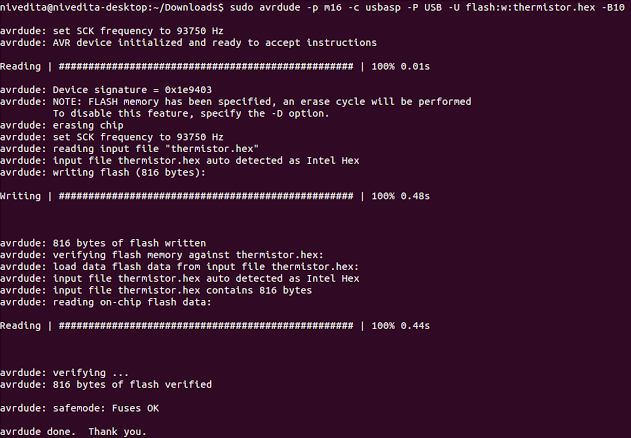
\includegraphics[scale=0.9]{usb.png}
\caption{Using USBASP as an ISP }
\end{figure}
\newpage
\subsubsection{Troubleshooting}
\hspace{12pt}\checkmark Check if the board is powered from the SMPS, if not, power it and try it once powered.

\vspace{12pt}

\checkmark Check if all the essential flags in the command line are incorporated, if not make the appropriate changes.

\vspace{12pt}

\checkmark Check if the FRC cable of the USBASP is not stranded in the midway, if so, replace it.

\vspace{12pt}

\checkmark If all these fail, check if the appropriate MOSI, MISO, SCK, RST and GND pins of the header are appropriately shorted with the ones of the IC and also that the controller firmly sits on the base.

\vspace{12pt}
\newpage
\subsection{RS232 as a Programmer}
To program the IC, we can also use DB9 connector via RS232 cable. The DB9 connector looks like the one below.\vspace{12pt} 
\begin{figure}[h!]
\centering
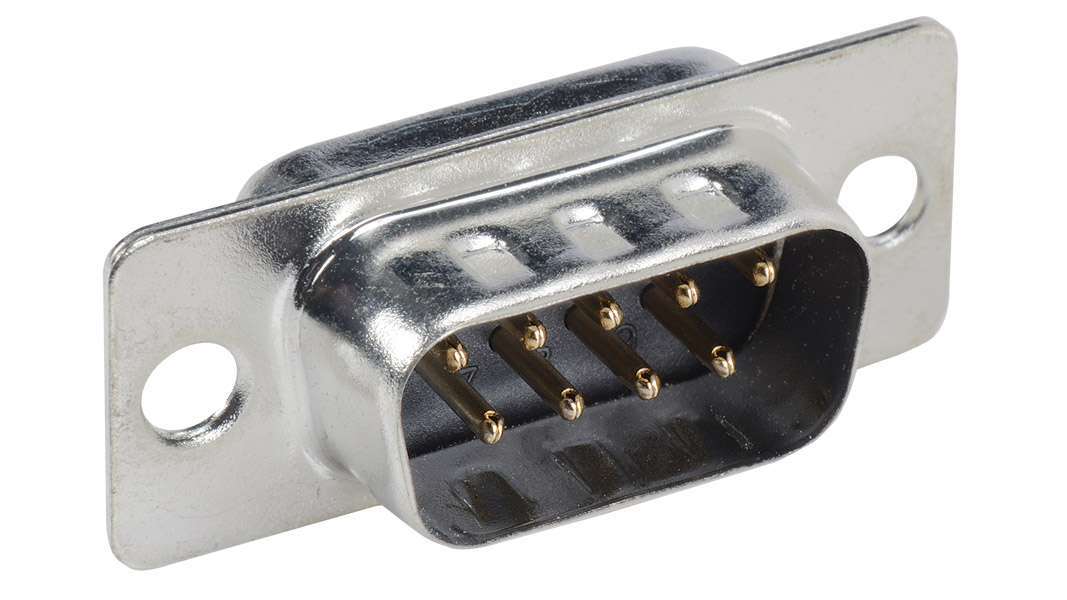
\includegraphics[scale=0.1]{DB9M.png}
\caption{DB9 connector}
\end{figure}


For programming the IC using DB9 connector via SPI protocol, we need yo build up some external circuitry first.

The circuit connections are done as the one shown below. This involves connecting some electrical components, which are in the end connected to the same 10 pin shrouded headers that are used for the USBASP as a programmer. In the programmer board the connections made are like the one shown below.
\vspace{12pt}
\begin{figure}[h!]
\centering
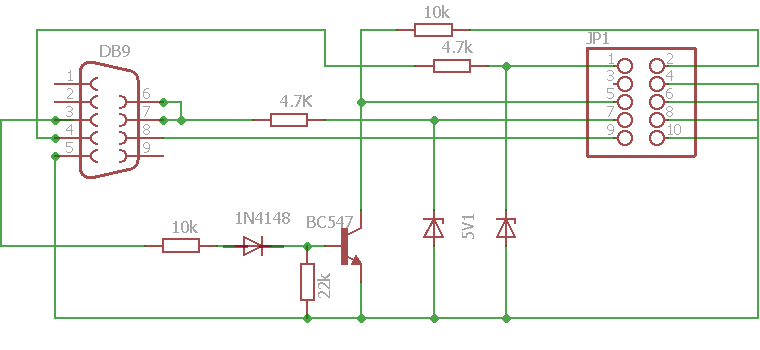
\includegraphics[scale=1]{Makedb9.png}
\caption{DB9 connector}
\end{figure}
\vspace{12pt}

Using DB-9 for the communication as per the RS-232 standard is chosen as the protocol is the oldest, easiest and doesn't require many hardware resources to be incorporated on the board for the IC to be programmed. As most of the present day systems like laptops may not have these ports, we can use a USB to RS-232 cable, which can be plugged into the USB port present on the system. 


\subsection{Programming using RS-232}
\vspace{12pt}
\hspace{17pt}Step 1: Connect the given RS-232 cable to the DB-9 port on the programmer board.

\vspace{12pt}
Step 2: You should open command line and then enter into the directory in which you have saved the HEX file compiled using LDMicro.  

\vspace{12pt}
Step 3: Now that all the things are ready, finally enter the following command on \texttt{Terminal}.\singlespace
\vspace{12pt}
\texttt{avrdude -p atmega16 -P /dev/ttyUSB0	-c ponyser -v -U flash:w:test1.hex}\linebreak\singlespace
\vspace{12pt}
\begin{figure}[h!]
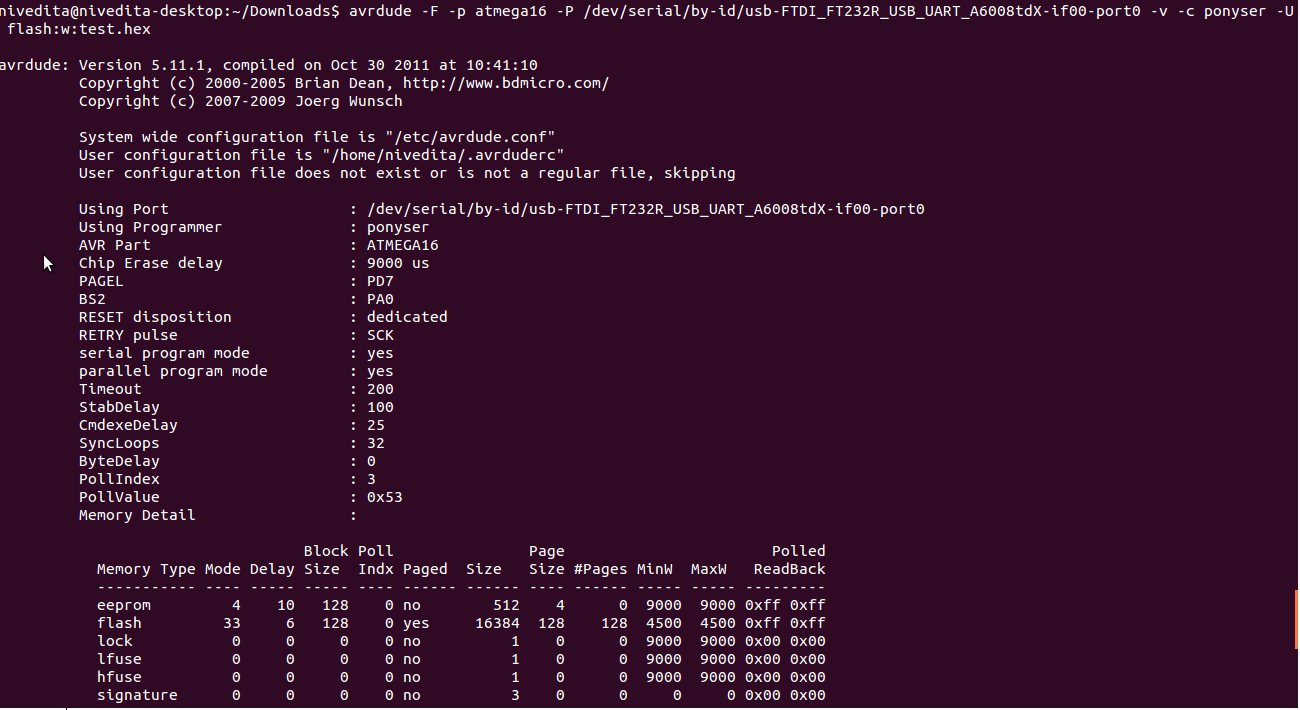
\includegraphics[scale=0.4]{RS1.png}
\end{figure}
\vspace{12pt}
\begin{figure}[h!]
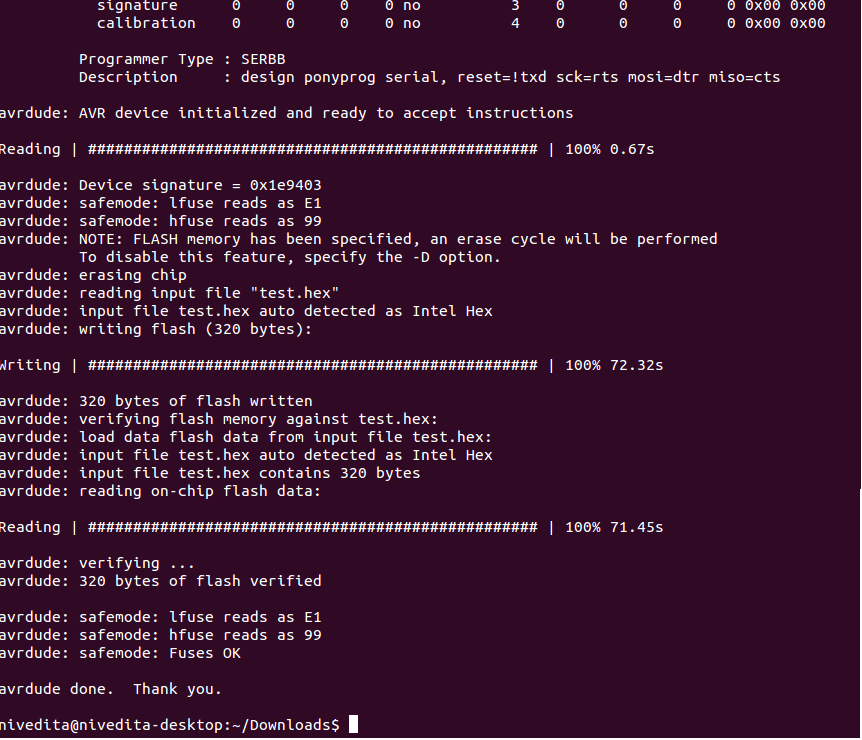
\includegraphics[scale=0.5]{RS2.png}
\caption{Programming via RS-232}
\end{figure}
\vspace{12pt}

This result is obtained if all the connections are fine. If only you obtain such a result, it means that the HEX code has been burnt onto the IC. If you obtain any other result, please look at the troubleshooting section.
\newpage
\subsubsection{Troubleshooting}
\vspace{12pt}
\hspace{12pt}\checkmark Check if the board is powered from the SMPS, if not, power it and try it once powered.

\vspace{12pt}

\checkmark Check if all the essential flags in the command line are incorporated, if not make the appropriate changes.

\vspace{12pt}

\checkmark Check if the RS-232 cable of the is connected securely to the DB9 connector.

\vspace{12pt}
\checkmark If all of this fails, then check if the reset pin of the microcontroller is at \texttt{+5 Volts} if not then externally connect it to \texttt{+5 Volts}.
\vspace{12pt}
\newpage
\subsection{Setting up the fuse bits}
Now that the programmer is installed on the system, we need to adjust the properties of the controller IC such that it meets the necessary requirements along with the peripherals installed on the board. Essentially, fuse bits are the ones that decide how the controller responds, like which clock frequency it responds to or its programming availabilities. Setting up the fuse is a crucial task as the controller may not respond later if the fuse bits that are set are not in accordance with the attached peripherals. Before setting the fuses, the factory settings on the controller make sure it works on the internal oscillator of clock speed 1MHz. It's mostly dependent on 2 fuses - lfuse and hfuse. Both of these have hex 8 bit values. When working on communication with the device, like UART, these fuse bits play a key role, if not defined, the controller works on the internal clock that's much slower than the external crystal. For the controller, 16MHz external crystal was selected. This meant the controller shall configure this external crystal and work on it.

\texttt{WARNING: Fuse bits control the way the controller responds. If any mistake is made in setting up the fuse bits, then the controller becomes isolated from the external circuit. This means that the controller doesn't respond and renders useless. Hence, always triple check before entering the fuse bits. This is the best practice, or else you may end up wasting one IC.}

\vspace{12pt} Type the following command into the \texttt{Terminal}:

\vspace{12pt}

For USBASP:
\vspace{12pt}

\texttt{sudo avrdude -p m16 -c usbasp -U lfuse:w:0xFF:m -U hfuse:w:0xD9:m -B10}\vspace{12pt}

For RS232:\vspace{12pt}


\texttt{avrdude -p m16 -c ponyser -P /dev/ttyUSB0 -U lfuse:w:0xFF:m -U hfuse:w:0xD9:m }\newpage

\begin{figure}[h!]
\centering
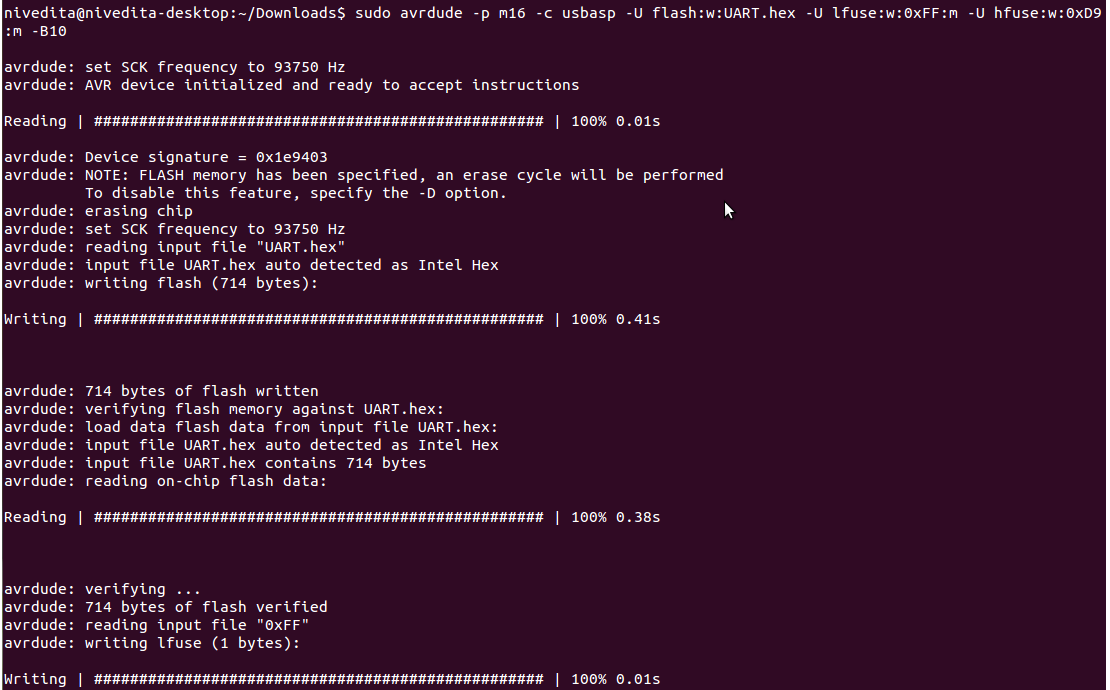
\includegraphics[scale=0.5]{fuse1.png}
\caption{Setting the fuse bits}
\end{figure}	 
\newpage
\begin{figure}
\centering
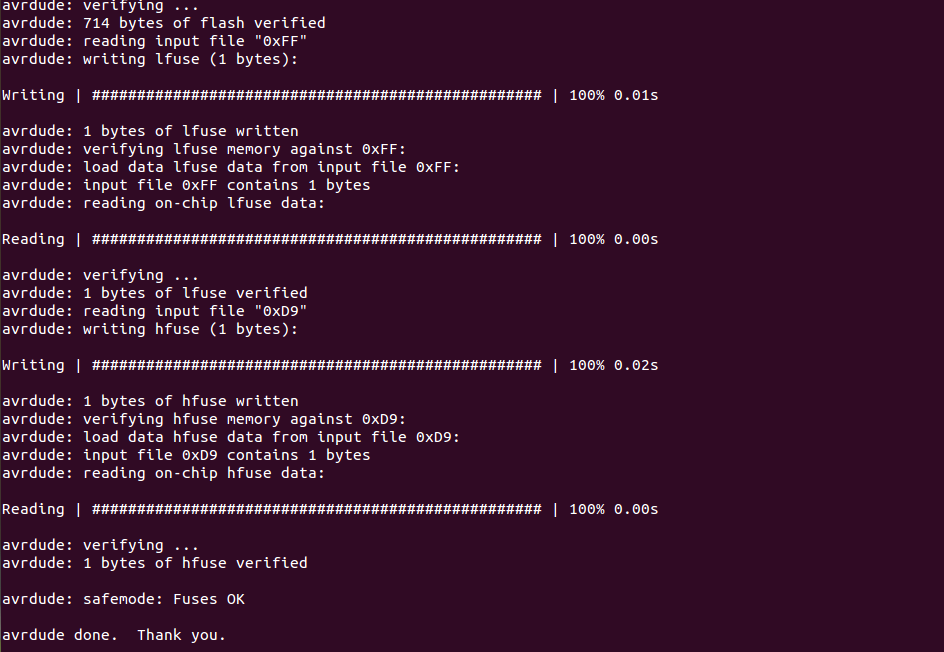
\includegraphics[scale=0.5]{fuse2.png}
\caption{Setting the fuse bits}
\end{figure}

Try to read the fuse bits after setting it. This will help you recognize if the IC has configured the external 16MHz crystal.\vspace{12pt}

If using USBASP enter : 

\vspace{12pt}

\texttt{avrdude -p m16 -C usb -P usbasp}

\vspace{12pt}

If using RS232 programmer enter :

\vspace{12pt}

\texttt{avrdude -p m16 -C /dev/ttyUSB0 -P ponyser}

\vspace{12pt}

You will get a screen like this :

You can see that the fuse bits are read off. This implies that the external crystal is working in sync with the controller. You can verify that the fuse bits are the ones that you set earlier. 

\newpage If such a reading doesn't come up, follow these steps:

\vspace{12pt}

\checkmark Check that the command line is proper and you have written the correct command line with all the necessary flags like the controller mentioned is correct.

\vspace{12pt}

\checkmark Make sure that the power supply is connected and the programmer i.e. USBASP or RS232 is configured and the correct programmer is mentioned in the command line

\vspace{12pt}

\checkmark Make sure that the controller is firmly connected to the IC base. If not press it so that it sits firmly.

\vspace{12pt}

\checkmark If these do not work, then remove the controller IC from the base and then remove the crystal and solder a new 16MHz crystal. Make sure that you do not heat the crystal extensively. Due to this there's usually a mismatch in the clock speeds.

\vspace{12pt}
\cleardoublepage
{\Large \section{Using UART function}}
UART basically is the most basic protocol for serially transmitting and receiving the data from the sensor. UART stands for Universal Asynchronous Receiver Transmitter.  The ladder logic allows us to program the UART facility easily in LD Micro. The values monitored in the ladder can be used to be displayed on the serial monitor. Say for example you have values that change with time and are varying, that is the value is analog, which means the values change over time and aren't discrete. Hence, monitoring the specific values become easy over the serial monitor. \vspace{12pt}

Setting up the UART is so easy. Just connect the TX near the MAX232 IC to pin 14 of the IC and connect RX near the MAX232 IC to pin 15 of the IC. Now in the ladder use the UART send feature. The variable associated with UART send part will be the value that you would want to monitor. Mostly these values being analog will be connected to analog pins i.e. pins of Port A. So, the variables associated with the analog values have Avar kind of a structure, when using that for UART, append the 'A' in front of the variable name. So the variable linked in the UART send part will be 'Avar' and not 'var'.\vspace{12pt} 

For looking at the associated values, install a serial monitor on the system. This is helpful to the the Raw data associated. When monitored, the values seen are hex in nature, they start with the '0x' part, which implies the code is hexadecimal. This is helpful for suggesting thresholds and creating a level for a particular application. The hex values are assigned like 0x00 to 0x3FF which means the values range from 0 to 1023. This means the values 0V is mapped to 0x00 and value 5V (maximum from the controller) will be assigned 0x3FF value. This is how the mapping will be done. 
\newpage
\end{document}

